\chapter{ダイナミクスの特徴づけ}\label{chap:analysis}

この章では, 第\ref{sec:simulation}章において行ったシミュレーションを用いて, ダイナミクスについて考える. 適宜文脈に則した画像を添付するが, 入りきらない部分は付録\ref{ap:analysis}に収録する.

また, 以降の議論は定常状態であるとみなした$t_i \sqrt{\varepsilon / m \sigma^2} = 4.0 \times 10^{4}$以降のデータを用いて行う.

\section{重心位置}\label{sec:CoM}

重心位置の標準偏差$\sigma (Y_g)$は以下のように書くことができる.

\begin{align}
  \sigma (Y_g) &= \sqrt{\frac{1}{N_{D}}\sum_{t=t_i}^{t=t_f} (Y_{g}(t) - \bar{Y_g})^2}
\end{align}

これは, 時間発展する重心位置のばらつき具合を意味する. 後述する空間的なばらつき$\sigma_{y} (t) (式\eqref{dis_field})$とは定義から見ても分かるとおり異なる量である.

\ref{sec:RaRtmap}節(重力と熱流を同時にかける)のシミュレーションで得たデータを用いて, 重心位置の標準偏差について, それぞれ横軸を変えて同時プロットで表す. 

\begin{figure}[H]
  \begin{tabular}{cc}
    \begin{minipage}[t]{0.5\hsize}
      \centering
      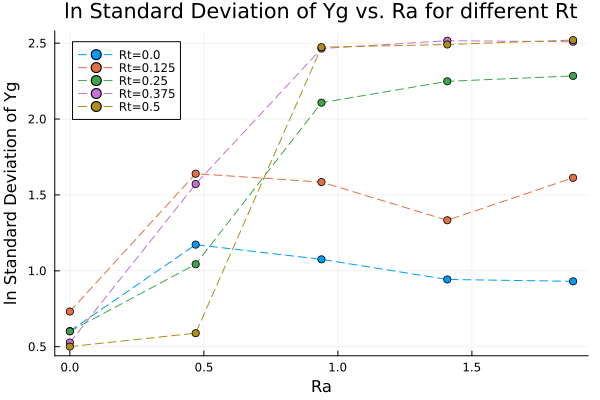
\includegraphics[width=\textwidth]{image/lnStdYg_Ra0.0to1.877538_Rt0.0to0.5_ti25000.png}
      \subcaption{横軸$\colon \text{R}_\text{a}$}
      \label{}
    \end{minipage}
    \begin{minipage}[t]{0.5\hsize}
      \centering
      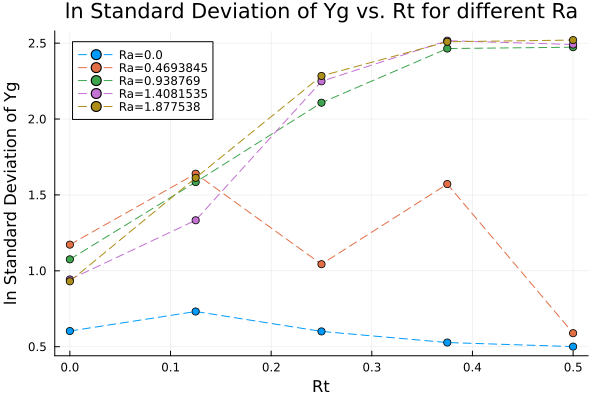
\includegraphics[width=\textwidth]{image/lnStdYg_Rt0.0to0.5_Ra0.0to1.877538_ti25000.png}
      \subcaption{横軸$\colon \text{R}_\text{t}$}
      \label{}
    \end{minipage}
  \end{tabular}
  \caption{縦軸:重心位置の標準偏差の対数プロット}
  \label{}
\end{figure}

\vspace{1\baselineskip}

図\ref{fig:RaRtmap_time_Ra0.469_Rt0.500}$\text{R}_\text{a} = 0.469, \text{R}_\text{t} = 0.5$と図\ref{fig:RaRtmap_time_Ra0.938_Rt0.500} $\text{R}_\text{a} = 0.938, \text{R}_\text{t} = 0.5$の間をより詳しく見る.

\begin{figure}[H]
  \centering
  \begin{tabular}{ccccc}
    \begin{minipage}[t]{0.2\hsize}
      \centering
      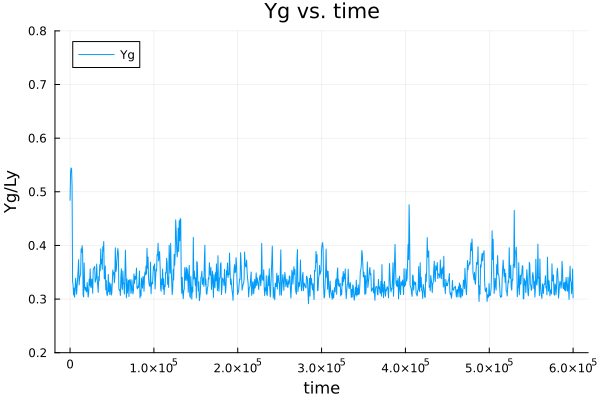
\includegraphics[width=\textwidth]{image/RaRtmap_time/2023-11-22T18:19:26.970_RaRt_chi1.265_Ay50_rho0.4_T0.43_dT0.04_Rd0.0_Rt0.5_Ra0.4693845_g0.0003999718779659611_run1.2e8.png}
      \subcaption{Ra0.4693845}
      \label{}
    \end{minipage} &
    \begin{minipage}[t]{0.2\hsize}
      \centering
      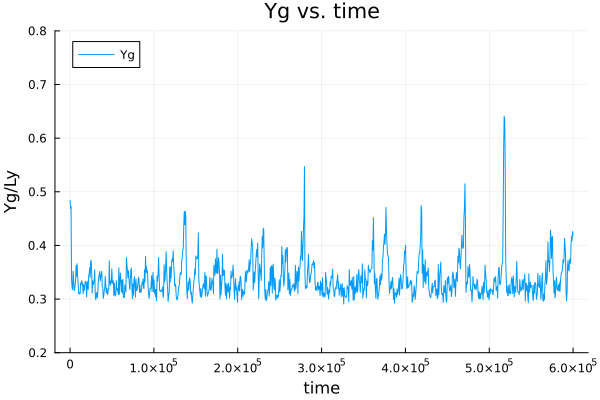
\includegraphics[width=\textwidth]{image/RaRtmap_time/2023-11-22T18:19:27.571_RaRt_chi1.265_Ay50_rho0.4_T0.43_dT0.04_Rd0.0_Rt0.5_Ra0.586730625_g0.0003999718779659611_run1.2e8.png}
      \subcaption{Ra0.586730625}
      \label{}
    \end{minipage} &
    \begin{minipage}[t]{0.2\hsize}
      \centering
      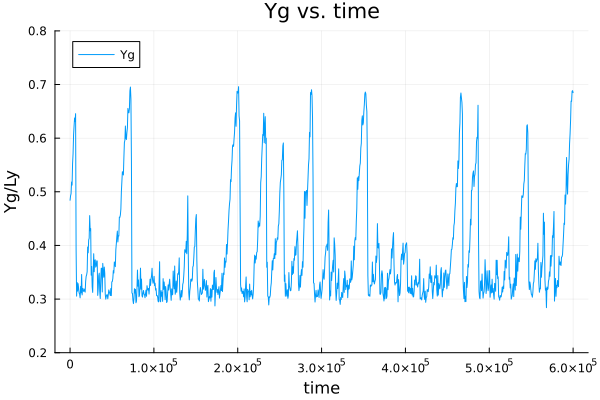
\includegraphics[width=\textwidth]{image/RaRtmap_time/2023-11-22T18:19:27.653_RaRt_chi1.265_Ay50_rho0.4_T0.43_dT0.04_Rd0.0_Rt0.5_Ra0.70407675_g0.0003999718779659611_run1.2e8.png}
      \subcaption{Ra0.70407675}
      \label{}
    \end{minipage} &
    \begin{minipage}[t]{0.2\hsize}
      \centering
      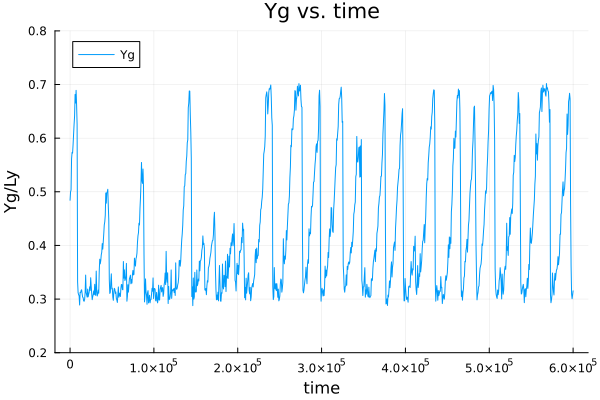
\includegraphics[width=\textwidth]{image/RaRtmap_time/2023-11-22T18:19:27.720_RaRt_chi1.265_Ay50_rho0.4_T0.43_dT0.04_Rd0.0_Rt0.5_Ra0.821422875_g0.0003999718779659611_run1.2e8.png}
      \subcaption{Ra0.821422875}
      \label{}
    \end{minipage} &
    \begin{minipage}[t]{0.2\hsize}
      \centering
      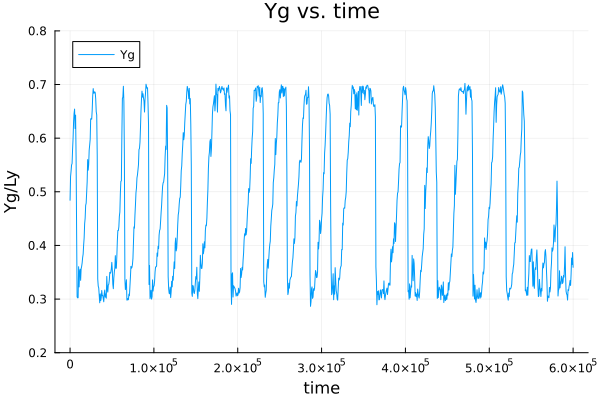
\includegraphics[width=\textwidth]{image/RaRtmap_time/2023-11-22T18:19:27.787_RaRt_chi1.265_Ay50_rho0.4_T0.43_dT0.04_Rd0.0_Rt0.5_Ra0.938769_g0.0003999718779659611_run1.2e8.png}
      \subcaption{Ra0.938769}
      \label{}
    \end{minipage} 
  \end{tabular}
  \caption{}
  \label{}
\end{figure}

\begin{figure}[H]
  \centering
  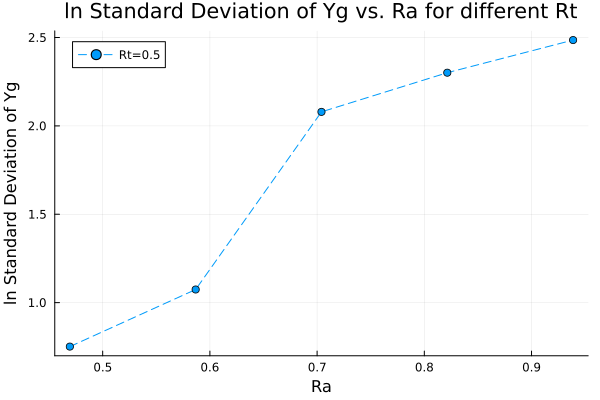
\includegraphics[scale=0.5]{image/lnStdYg_Ra0.4693845to0.98769_Rt0.5_ti25000.png}
  \caption{横軸:$\text{R}_\text{a}$, 縦軸:重心位置の標準偏差の対数プロット}
  \label{}
\end{figure}

\vspace{1\baselineskip}

図\ref{fig:Ra0.70407675Rt0.5}$\text{R}_\text{a} = 0.469, \text{R}_\text{t} = 0.5$と図\ref{fig:Ra0.938769Rt0.5} $\text{R}_\text{a} = 0.938, \text{R}_\text{t} = 0.5$の間を詳しく見る. 

% \begin{figure}[H]
%   \centering
%   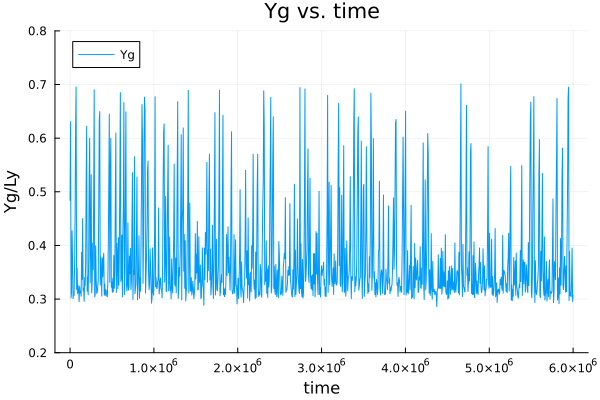
\includegraphics[scale=0.6]{image/RaRtmap_time/2023-11-27T01:34:51.948_Ra_chi1.265_Ay50_rho0.4_T0.43_dT0.04_Rd0.0_Rt0.5_Ra0.70407675_g0.0003999718779659611_run1.2e9.png}
%   \caption{Ra0.4693845}
%   \label{}
% \end{figure}

\begin{figure}[H]
  \centering
  \begin{tabular}{ccccc}
    \begin{minipage}[t]{0.2\hsize}
      \centering
      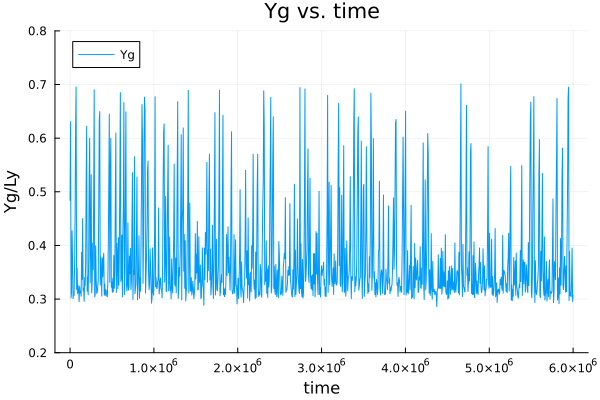
\includegraphics[width=\textwidth]{image/RaRtmap_time/2023-11-27T01:34:51.948_Ra_chi1.265_Ay50_rho0.4_T0.43_dT0.04_Rd0.0_Rt0.5_Ra0.70407675_g0.0003999718779659611_run1.2e9.png}
      \subcaption{Ra0.70407675}
      \label{}
    \end{minipage} &
    \begin{minipage}[t]{0.2\hsize}
      \centering
      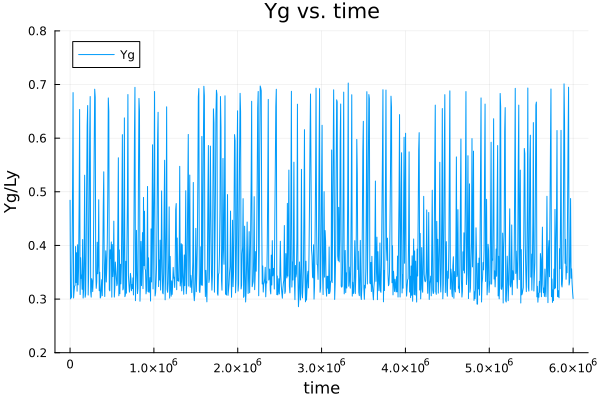
\includegraphics[width=\textwidth]{image/RaRtmap_time/2023-11-27T01:34:52.442_Ra_chi1.265_Ay50_rho0.4_T0.43_dT0.04_Rd0.0_Rt0.5_Ra0.7627498125_g0.0003999718779659611_run1.2e9.png}
      \subcaption{Ra0.7627498125}
      \label{}
    \end{minipage} &
    \begin{minipage}[t]{0.2\hsize}
      \centering
      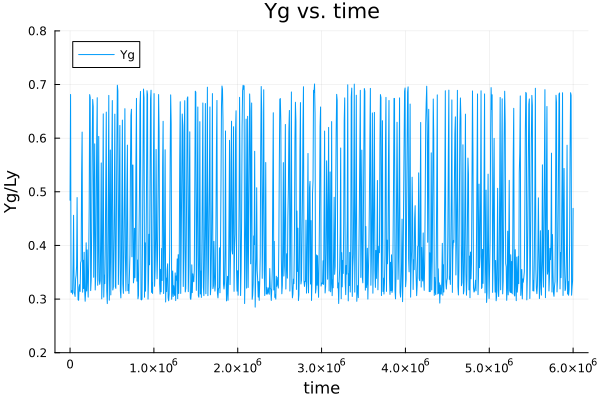
\includegraphics[width=\textwidth]{image/RaRtmap_time/2023-11-27T01:34:52.545_Ra_chi1.265_Ay50_rho0.4_T0.43_dT0.04_Rd0.0_Rt0.5_Ra0.821422875_g0.0003999718779659611_run1.2e9.png}
      \subcaption{Ra0.821422875}
      \label{}
    \end{minipage} &
    \begin{minipage}[t]{0.2\hsize}
      \centering
      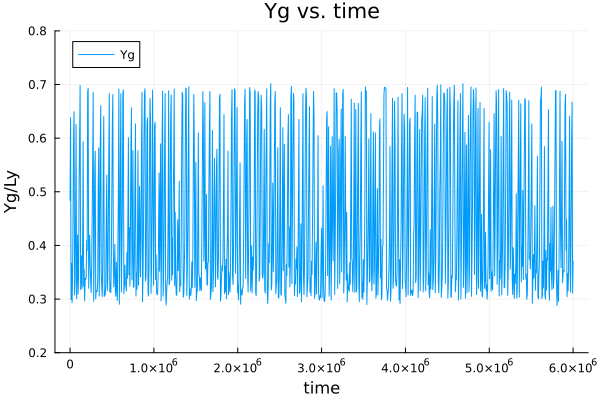
\includegraphics[width=\textwidth]{image/RaRtmap_time/2023-11-27T01:34:52.610_Ra_chi1.265_Ay50_rho0.4_T0.43_dT0.04_Rd0.0_Rt0.5_Ra0.8800959375_g0.0003999718779659611_run1.2e9.png}
      \subcaption{Ra0.8800959375}
      \label{}
    \end{minipage} &
    \begin{minipage}[t]{0.2\hsize}
      \centering
      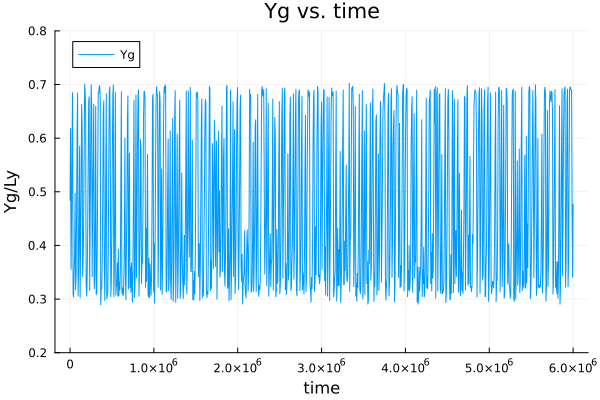
\includegraphics[width=\textwidth]{image/RaRtmap_time/2023-11-27T01:34:52.675_Ra_chi1.265_Ay50_rho0.4_T0.43_dT0.04_Rd0.0_Rt0.5_Ra0.938769_g0.0003999718779659611_run1.2e9.png}
      \subcaption{Ra0.938769}
      \label{}
    \end{minipage} 
  \end{tabular}
  \caption{$t_i = 0 , t_f = 6.0 \times 10^6, t\sqrt{\epsilon/m{\sigma}^2} = 6000$ごとにプロット.}
  \label{}
\end{figure}

\begin{figure}[H]
  \centering
  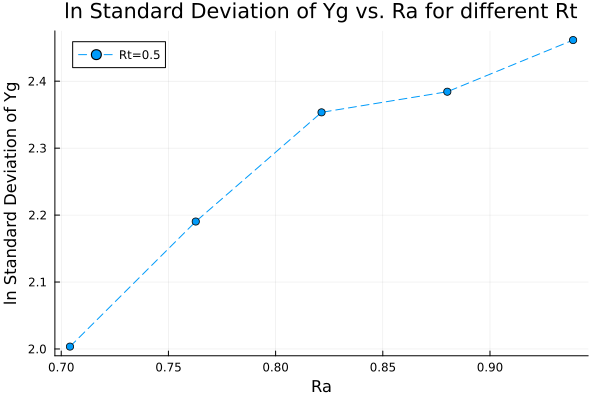
\includegraphics[scale=0.5]{image/lnStdYg_Ra0.70407675to0.98769_Rt0.5_ti25000.png}
  \caption{横軸:$\text{R}_\text{a}$, 縦軸:重心位置の標準偏差の対数プロット}
  \label{}
\end{figure}

\vspace{1\baselineskip}

先の分析では, 時間プロットの幅が大きい可能性があるため, 図\ref{fig:RaRtmap_time_Ra0.469_Rt0.500}$\text{R}_\text{a} = 0.469, \text{R}_\text{t} = 0.5$と図\ref{fig:RaRtmap_time_Ra0.938_Rt0.500} $\text{R}_\text{a} = 0.938, \text{R}_\text{a} = 0.5$の間のプロット幅を小さくしたデータを使う. その際, 簡単のため, $\text{R}_\text{a} =0.5 \sim 1.0$の間を見ることにする.

\begin{figure}[H]
  \centering
  \begin{tabular}{ccccc}
    \begin{minipage}[t]{0.2\hsize}
      \centering
      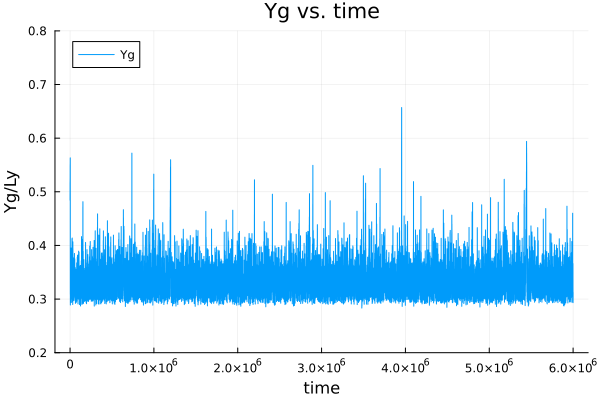
\includegraphics[width=\textwidth]{image/RaRtmap_time/2023-11-30T20:13:31.872_Ra_chi1.265_Ay50_rho0.4_T0.43_dT0.04_Rd0.0_Rt0.5_Ra0.5_g0.0003999718779659611_run1.2e9.png}
      \subcaption{Ra0.5}
      \label{}
    \end{minipage} &
    \begin{minipage}[t]{0.2\hsize}
      \centering
      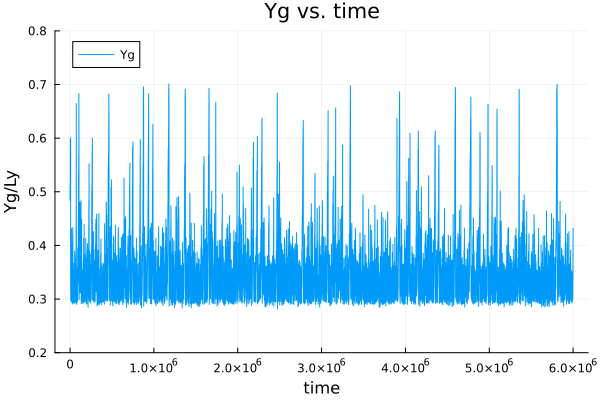
\includegraphics[width=\textwidth]{image/RaRtmap_time/2023-11-30T20:13:32.405_Ra_chi1.265_Ay50_rho0.4_T0.43_dT0.04_Rd0.0_Rt0.5_Ra0.625_g0.0003999718779659611_run1.2e9.png}
      \subcaption{Ra0.625}
      \label{}
    \end{minipage} &
    \begin{minipage}[t]{0.2\hsize}
      \centering
      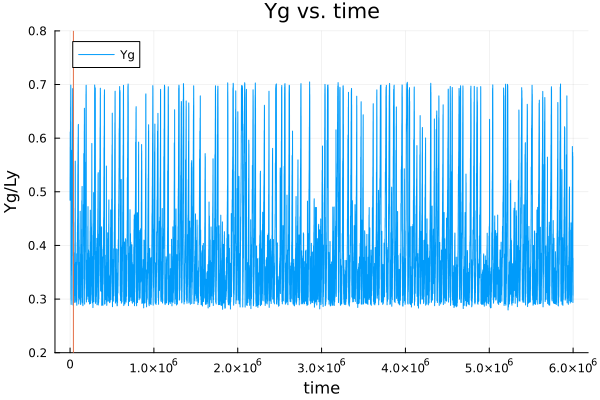
\includegraphics[width=\textwidth]{image/RaRtmap_time/2023-11-30T20:13:32.471_Ra_chi1.265_Ay50_rho0.4_T0.43_dT0.04_Rd0.0_Rt0.5_Ra0.75_g0.0003999718779659611_run1.2e9.png}
      \subcaption{Ra0.75}
      \label{}
    \end{minipage} &
    \begin{minipage}[t]{0.2\hsize}
      \centering
      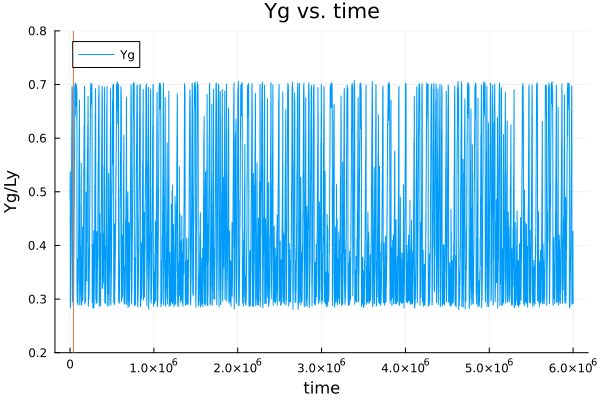
\includegraphics[width=\textwidth]{image/RaRtmap_time/2023-11-30T20:13:32.545_Ra_chi1.265_Ay50_rho0.4_T0.43_dT0.04_Rd0.0_Rt0.5_Ra0.875_g0.0003999718779659611_run1.2e9.png}
      \subcaption{Ra0.875}
      \label{}
    \end{minipage} &
    \begin{minipage}[t]{0.2\hsize}
      \centering
      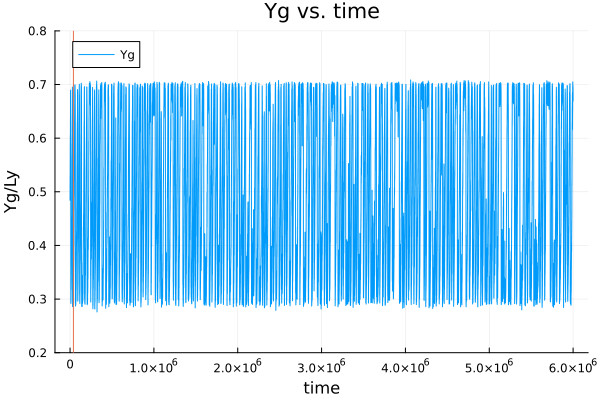
\includegraphics[width=\textwidth]{image/RaRtmap_time/2023-11-30T20:13:32.620_Ra_chi1.265_Ay50_rho0.4_T0.43_dT0.04_Rd0.0_Rt0.5_Ra1.0_g0.0003999718779659611_run1.2e9.png}
      \subcaption{Ra1.0}
      \label{}
    \end{minipage} 
  \end{tabular}
  \caption{}
  \label{}
\end{figure}

\begin{figure}[H]
  \centering
  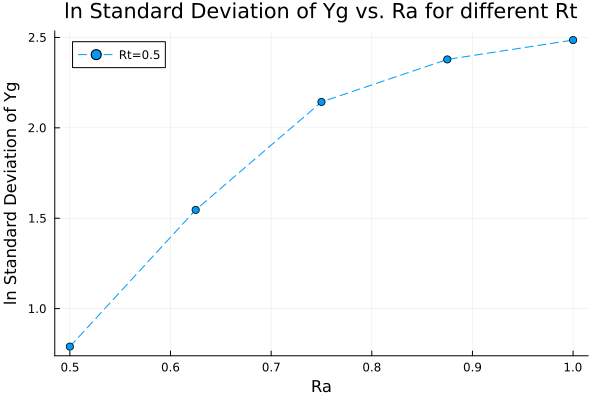
\includegraphics[scale=0.5]{image/lnStdYg_Ra0.5to1.0_Rt0.5_ti25000.png}
  \caption{横軸:$\text{R}_\text{a}$, 縦軸:重心位置の標準偏差の対数プロット}
  \label{fig:lnStdYg_Ra0.5to1.0_Rt0.5_ti25000}
\end{figure}

図\ref{fig:lnStdYg_Ra0.5to1.0_Rt0.5_ti25000}からも見て分かるように, $\text{R}_\text{t} = 0.5$において, $\text{R}_\text{a}$ の値を大きくするほど, 各系の重心位置の時間発展はばらつきが大きくなると言うことがわかる.

\section{リミットサイクル}\label{sec:limitcycle}

周期的なダイナミクスが見える系について考える. 非線形振動にはリミットサイクル振動\cite{Rhythm}と呼ばれる振動の形態がある. ここでは流体系の重心位置と空間的なばらつきの相空間での軌道をみることにする.

流体系の空間的なばらつき$\sigma_{y} (t)$を以下のように定義する.

\begin{align}
  \label{dis_field}
  \sigma_{y} (t)
  &\equiv \sqrt{\frac{1}{N} \sum_{i=1}^{N} (y_i (t) - \bar{y_i}(t) )^2} \\
  &= \sqrt{\frac{1}{N} \sum_{i=1}^{N} (y_i (t) - Y_g (t) )^2} 
  % &= \sqrt{\frac{1}{N} \sum_{i=1}^{N} {{y_i} (t)}^2 - {{Y_g} (t)}^2}
\end{align}

\ref{sec:RaRtmap10}節(重力と熱流を同時にかける(時間10倍))で得たデータを用いて, 重心位置と, 流体系の空間的なばらつきの時系列プロットをそれぞれ並べる.

まず, $\text{R}_\text{a}$を固定して, $\text{R}_\text{t}$のみを変えた系での各物理量の時系列プロットを示す. 


\begin{figure}[H]
  \centering
  \begin{tabular}{ccc}
    \begin{minipage}[t]{0.3\hsize}
      \centering
      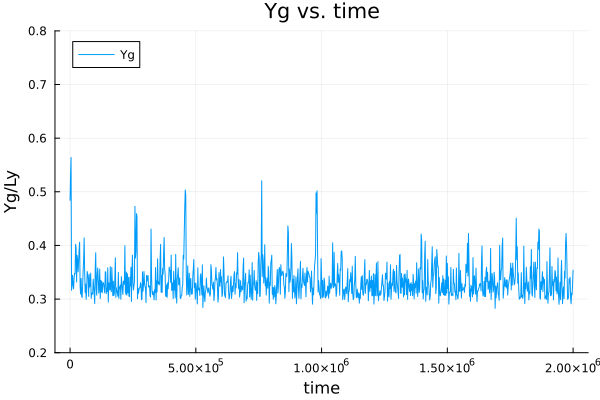
\includegraphics[width=\textwidth]{image/RaRtmap10_time/2023-12-28T12:38:51.436_map_10times_chi1.265_Ay50_rho0.4_T0.43_dT0.04_Rd0.0_Rt0.0_Ra1.877538_g0.0003999718779659611_run4.0e8.png}
      \subcaption{Ra1.877,Rt0.0}
      \label{}
    \end{minipage} &
    \begin{minipage}[t]{0.3\hsize}
      \centering
      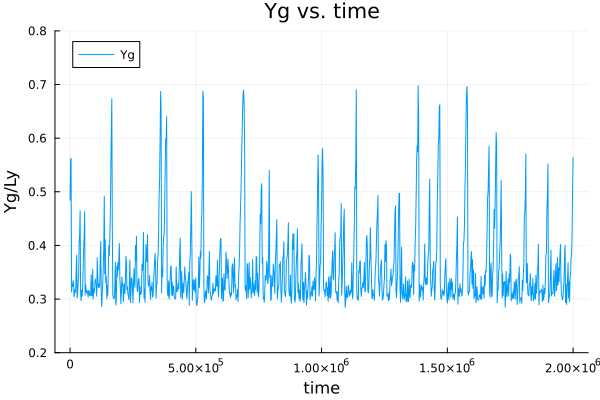
\includegraphics[width=\textwidth]{image/RaRtmap10_time/2023-12-28T12:38:51.827_map_10times_chi1.265_Ay50_rho0.4_T0.43_dT0.04_Rd0.0_Rt0.125_Ra1.877538_g0.0003999718779659611_run4.0e8.png}
      \subcaption{Ra1.877,Rt0.125}
      \label{}
    \end{minipage} &
    \begin{minipage}[t]{0.3\hsize}
      \centering
      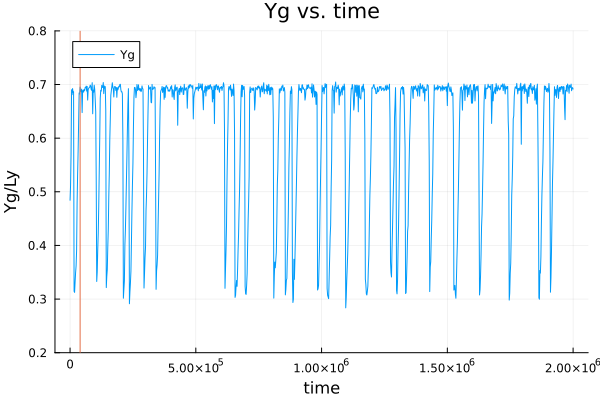
\includegraphics[width=\textwidth]{image/RaRtmap10_time/2023-12-28T12:38:52.986_map_10times_chi1.265_Ay50_rho0.4_T0.43_dT0.04_Rd0.0_Rt0.5_Ra1.877538_g0.0003999718779659611_run4.0e8.png}
      \subcaption{Ra1.877,Rt0.5}
      \label{}
    \end{minipage} 
  \end{tabular}
  \caption{重心位置の時系列プロット, $t_i = 4.0 \times 10^4 , t_f = 2.0 \times 10^6, t\sqrt{\epsilon/m{\sigma}^2} = 2000$ごとにプロット.}
  \label{}
\end{figure}

\begin{figure}[H]
  \centering
  \begin{tabular}{ccc}
    \begin{minipage}[t]{0.3\hsize}
      \centering
      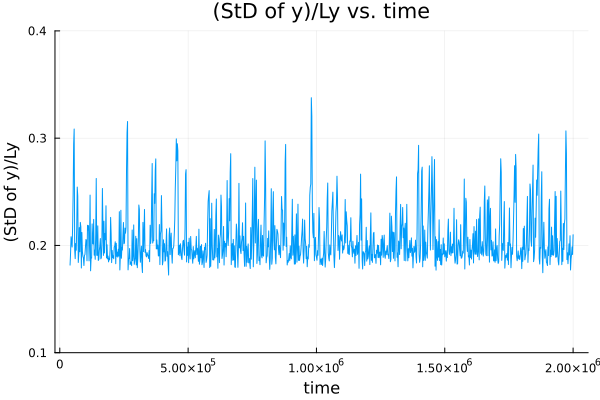
\includegraphics[width=\textwidth]{image/RaRtmap10_stdy/2023-12-28T12:38:51.436_map_10times_chi1.265_Ay50_rho0.4_T0.43_dT0.04_Rd0.0_Rt0.0_Ra1.877538_g0.0003999718779659611_run4.0e8.png}
      \subcaption{Ra1.877,Rt0.0}
      \label{}
    \end{minipage} &
    \begin{minipage}[t]{0.3\hsize}
      \centering
      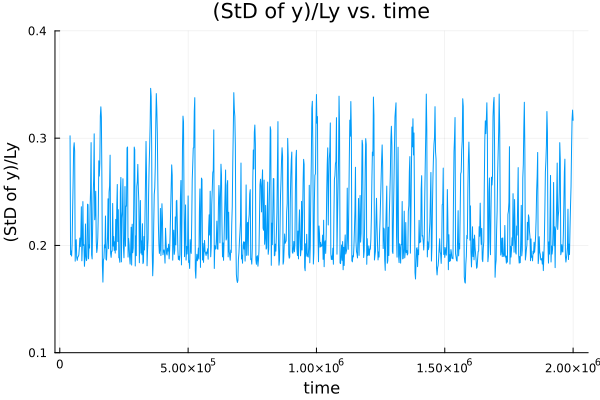
\includegraphics[width=\textwidth]{image/RaRtmap10_stdy/2023-12-28T12:38:51.827_map_10times_chi1.265_Ay50_rho0.4_T0.43_dT0.04_Rd0.0_Rt0.125_Ra1.877538_g0.0003999718779659611_run4.0e8.png}
      \subcaption{Ra1.877,Rt0.125}
      \label{}
    \end{minipage} &
    \begin{minipage}[t]{0.3\hsize}
      \centering
      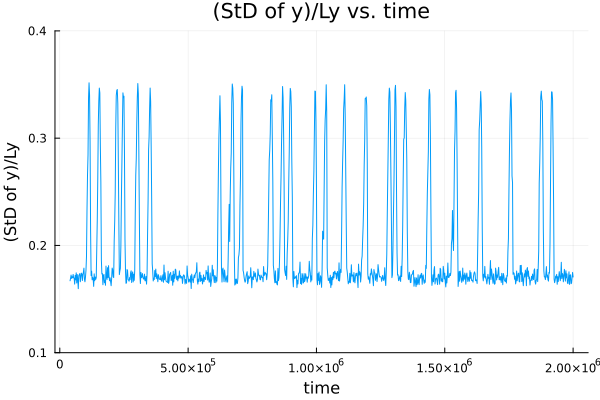
\includegraphics[width=\textwidth]{image/RaRtmap10_stdy/2023-12-28T12:38:52.986_map_10times_chi1.265_Ay50_rho0.4_T0.43_dT0.04_Rd0.0_Rt0.5_Ra1.877538_g0.0003999718779659611_run4.0e8.png}
      \subcaption{Ra1.877,Rt0.5}
      \label{}
    \end{minipage} 
  \end{tabular}
  \caption{流体系の空間的なばらつきの時系列プロット, $t_i = 4.0 \times 10^4 , t_f = 2.0 \times 10^6, t\sqrt{\epsilon/m{\sigma}^2} = 2000$ごとにプロット.}
  \label{}
\end{figure}

\vspace{1\baselineskip}

次に, $\text{R}_\text{t}$を固定して, $\text{R}_\text{a}$のみを変えた系での各物理量の時系列プロットを示す. 


\begin{figure}[H]
  \centering
  \begin{tabular}{ccc}
    \begin{minipage}[t]{0.3\hsize}
      \centering
      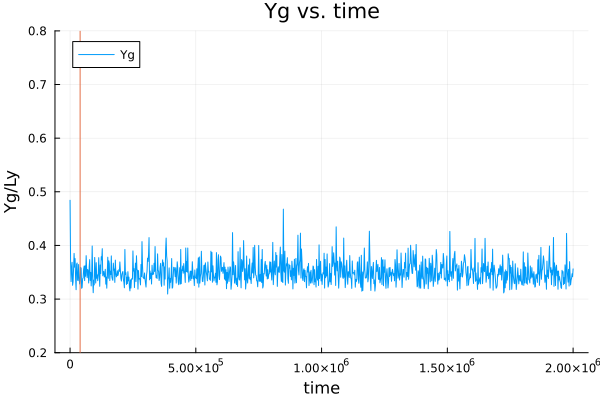
\includegraphics[width=\textwidth]{image/RaRtmap10_time/2023-12-28T12:38:52.686_map_10times_chi1.265_Ay50_rho0.4_T0.43_dT0.04_Rd0.0_Rt0.5_Ra0.0_g0.0003999718779659611_run4.0e8.png}
      \subcaption{Ra0.0,Rt0.5}
      \label{}
    \end{minipage} &
    \begin{minipage}[t]{0.3\hsize}
      \centering
      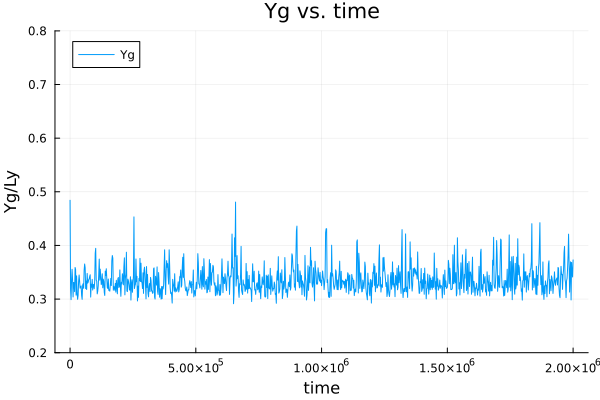
\includegraphics[width=\textwidth]{image/RaRtmap10_time/2023-12-28T12:38:52.752_map_10times_chi1.265_Ay50_rho0.4_T0.43_dT0.04_Rd0.0_Rt0.5_Ra0.4693845_g0.0003999718779659611_run4.0e8.png}
      \subcaption{Ra0.469,Rt0.5}
      \label{}
    \end{minipage} &
    \begin{minipage}[t]{0.3\hsize}
      \centering
      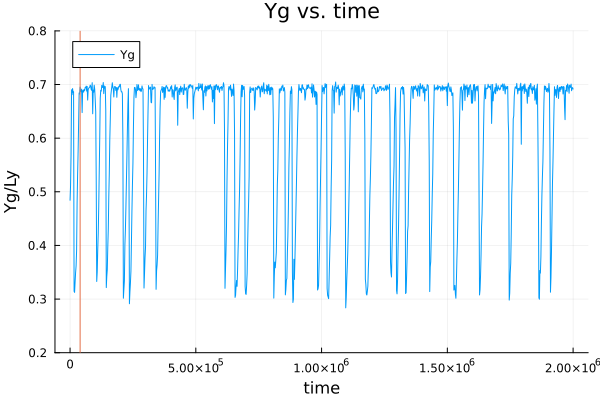
\includegraphics[width=\textwidth]{image/RaRtmap10_time/2023-12-28T12:38:52.986_map_10times_chi1.265_Ay50_rho0.4_T0.43_dT0.04_Rd0.0_Rt0.5_Ra1.877538_g0.0003999718779659611_run4.0e8.png}
      \subcaption{Ra1.877,Rt0.5}
      \label{}
    \end{minipage} 
  \end{tabular}
  \caption{重心位置の時系列プロット, $t_i = 4.0 \times 10^4 , t_f = 2.0 \times 10^6, t\sqrt{\epsilon/m{\sigma}^2} = 2000$ごとにプロット.}
  \label{}
\end{figure}

\begin{figure}[H]
  \centering
  \begin{tabular}{ccc}
    \begin{minipage}[t]{0.3\hsize}
      \centering
      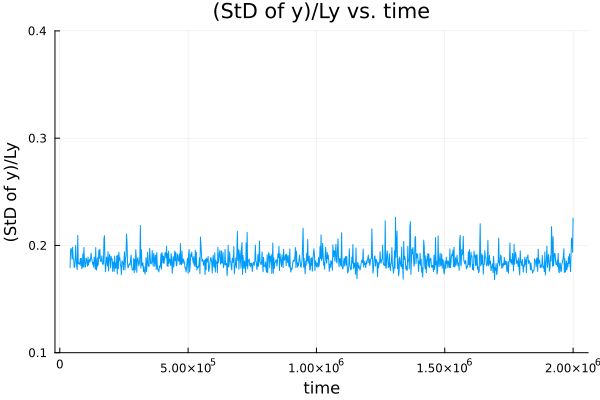
\includegraphics[width=\textwidth]{image/RaRtmap10_stdy/2023-12-28T12:38:52.686_map_10times_chi1.265_Ay50_rho0.4_T0.43_dT0.04_Rd0.0_Rt0.5_Ra0.0_g0.0003999718779659611_run4.0e8.png}
      \subcaption{Ra0.0,Rt0.5}
      \label{}
    \end{minipage} &
    \begin{minipage}[t]{0.3\hsize}
      \centering
      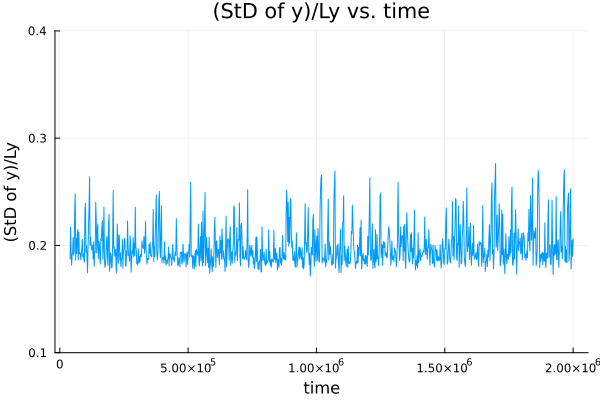
\includegraphics[width=\textwidth]{image/RaRtmap10_stdy/2023-12-28T12:38:52.752_map_10times_chi1.265_Ay50_rho0.4_T0.43_dT0.04_Rd0.0_Rt0.5_Ra0.4693845_g0.0003999718779659611_run4.0e8.png}
      \subcaption{Ra0.469,Rt0.5}
      \label{}
    \end{minipage} &
    \begin{minipage}[t]{0.3\hsize}
      \centering
      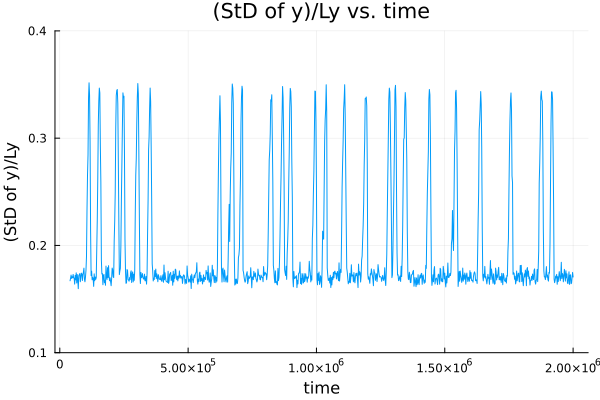
\includegraphics[width=\textwidth]{image/RaRtmap10_stdy/2023-12-28T12:38:52.986_map_10times_chi1.265_Ay50_rho0.4_T0.43_dT0.04_Rd0.0_Rt0.5_Ra1.877538_g0.0003999718779659611_run4.0e8.png}
      \subcaption{Ra1.877,Rt0.5}
      \label{}
    \end{minipage} 
  \end{tabular}
  \caption{流体系の空間的なばらつきの時系列プロット, $t_i = 4.0 \times 10^4 , t_f = 2.0 \times 10^6, t\sqrt{\epsilon/m{\sigma}^2} = 2000$ごとにプロット.}
  \label{}
\end{figure}

\vspace{1\baselineskip}

これらを踏まえて,流体系の重心位置と空間的なばらつきの相空間での軌道をそれぞれ並べる.


\begin{figure}[H]
  \centering
  \begin{tabular}{ccc}
    \begin{minipage}[t]{0.3\hsize}
      \centering
      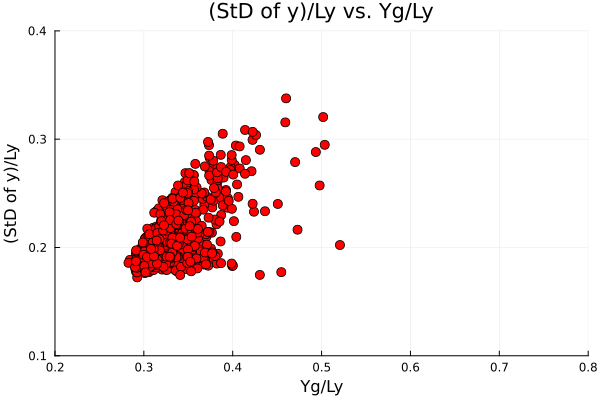
\includegraphics[width=\textwidth]{image/RaRtmap10_cycle/2023-12-28T12:38:51.436_map_10times_chi1.265_Ay50_rho0.4_T0.43_dT0.04_Rd0.0_Rt0.0_Ra1.877538_g0.0003999718779659611_run4.0e8.png}
      \subcaption{Ra1.877,Rt0.0}
      \label{}
    \end{minipage} &
    \begin{minipage}[t]{0.3\hsize}
      \centering
      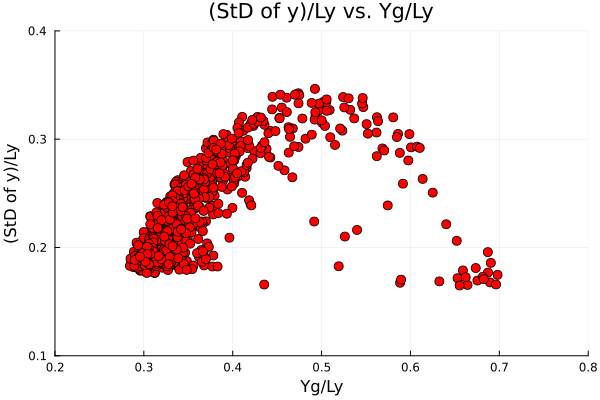
\includegraphics[width=\textwidth]{image/RaRtmap10_cycle/2023-12-28T12:38:51.827_map_10times_chi1.265_Ay50_rho0.4_T0.43_dT0.04_Rd0.0_Rt0.125_Ra1.877538_g0.0003999718779659611_run4.0e8.png}
      \subcaption{Ra1.877,Rt0.125}
      \label{}
    \end{minipage} &
    \begin{minipage}[t]{0.3\hsize}
      \centering
      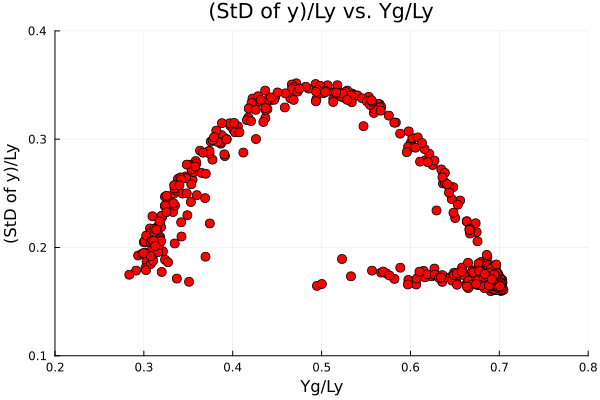
\includegraphics[width=\textwidth]{image/RaRtmap10_cycle/2023-12-28T12:38:52.986_map_10times_chi1.265_Ay50_rho0.4_T0.43_dT0.04_Rd0.0_Rt0.5_Ra1.877538_g0.0003999718779659611_run4.0e8.png}
      \subcaption{Ra1.877,Rt0.5}
      \label{}
    \end{minipage} 
  \end{tabular}
  \caption{リミットサイクル, Ra固定 $t_i = 4.0 \times 10^4 , t_f = 2.0 \times 10^6, t\sqrt{\epsilon/m{\sigma}^2} = 2000$ごとにプロット.}
  \label{fig:limitcycle_Ra}
\end{figure}

\begin{figure}[H]
  \centering
  \begin{tabular}{ccc}
    \begin{minipage}[t]{0.3\hsize}
      \centering
      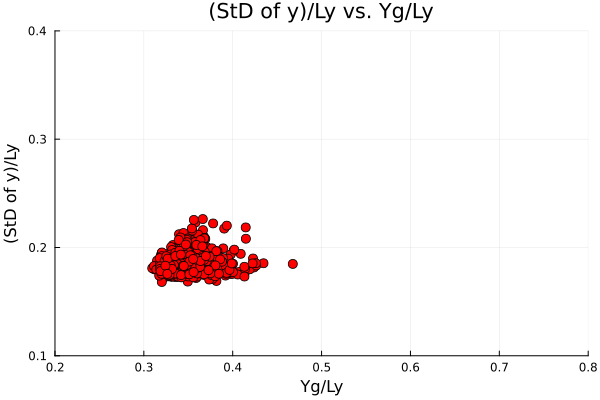
\includegraphics[width=\textwidth]{image/RaRtmap10_cycle/2023-12-28T12:38:52.686_map_10times_chi1.265_Ay50_rho0.4_T0.43_dT0.04_Rd0.0_Rt0.5_Ra0.0_g0.0003999718779659611_run4.0e8.png}
      \subcaption{Ra0.0,Rt0.5}
      \label{}
    \end{minipage} &
    \begin{minipage}[t]{0.3\hsize}
      \centering
      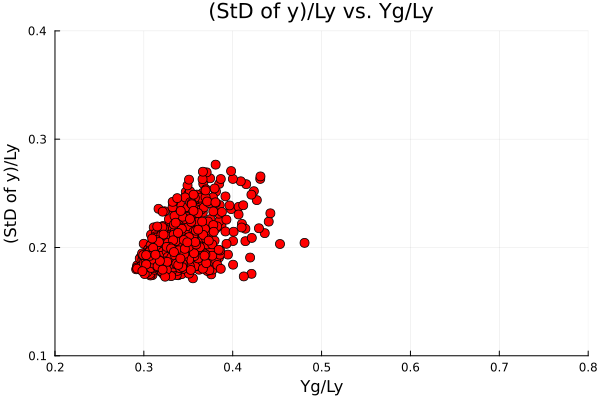
\includegraphics[width=\textwidth]{image/RaRtmap10_cycle/2023-12-28T12:38:52.752_map_10times_chi1.265_Ay50_rho0.4_T0.43_dT0.04_Rd0.0_Rt0.5_Ra0.4693845_g0.0003999718779659611_run4.0e8.png}
      \subcaption{Ra0.469,Rt0.5}
      \label{}
    \end{minipage} &
    \begin{minipage}[t]{0.3\hsize}
      \centering
      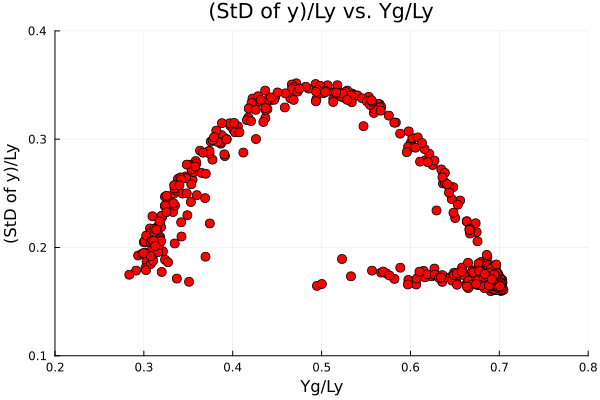
\includegraphics[width=\textwidth]{image/RaRtmap10_cycle/2023-12-28T12:38:52.986_map_10times_chi1.265_Ay50_rho0.4_T0.43_dT0.04_Rd0.0_Rt0.5_Ra1.877538_g0.0003999718779659611_run4.0e8.png}
      \subcaption{Ra1.877,Rt0.5}
      \label{}
    \end{minipage} 
  \end{tabular}
  \caption{リミットサイクル, Rt固定, $t_i = 4.0 \times 10^4 , t_f = 2.0 \times 10^6, t\sqrt{\epsilon/m{\sigma}^2} = 2000$ごとにプロット.}
  \label{fig:limitcycle_Rt}
\end{figure}

図\ref{fig:limitcycle_Ra}, \ref{fig:limitcycle_Rt}を見ると, 壁の濡れ性を強くするとサイクルが閉じ, このとき非定常で周期的なダイナミクスが現れているということがわかる.

また, このリミットサイクルからは, 周期的なダイナミクスが見れる系においては流体系が液滴を形成しつつ, 上壁に吸着しきるまでのスピードが, 液体の落下のそれよりも遅いことも分かる.

リミットサイクルのプロットが多く密集している箇所が濃くなるようにヒートマップを作ると以下のように, 系によって流体系が一定の位置に長く留まることが分かりやすくなる.

\begin{figure}[H]
  \centering
  \begin{tabular}{c}
    \begin{minipage}[t]{0.7\hsize}
      \centering
      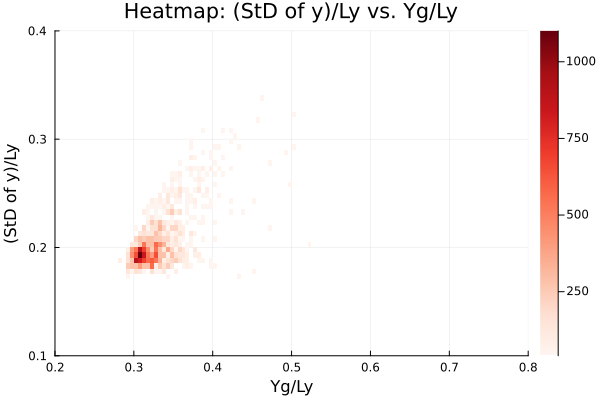
\includegraphics[width=\textwidth]{image/RaRtmap10_heat/2023-12-28T12:38:51.436_map_10times_chi1.265_Ay50_rho0.4_T0.43_dT0.04_Rd0.0_Rt0.0_Ra1.877538_g0.0003999718779659611_run4.0e8.png}
      \subcaption{Ra1.877,Rt0.0}
      \label{}
    \end{minipage} \\
    \begin{minipage}[t]{0.7\hsize}
      \centering
      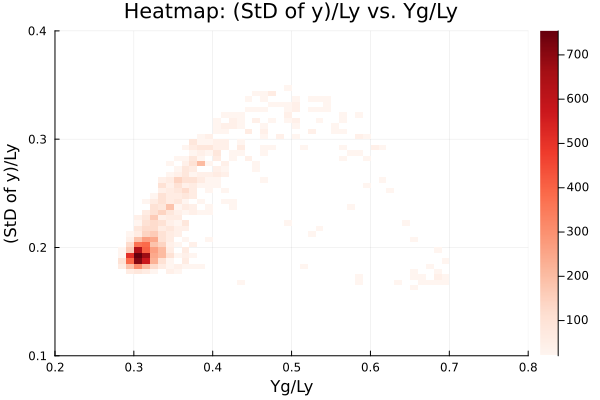
\includegraphics[width=\textwidth]{image/RaRtmap10_heat/2023-12-28T12:38:51.827_map_10times_chi1.265_Ay50_rho0.4_T0.43_dT0.04_Rd0.0_Rt0.125_Ra1.877538_g0.0003999718779659611_run4.0e8.png}
      \subcaption{Ra1.877,Rt0.125}
      \label{}
    \end{minipage} \\
    \begin{minipage}[t]{0.7\hsize}
      \centering
      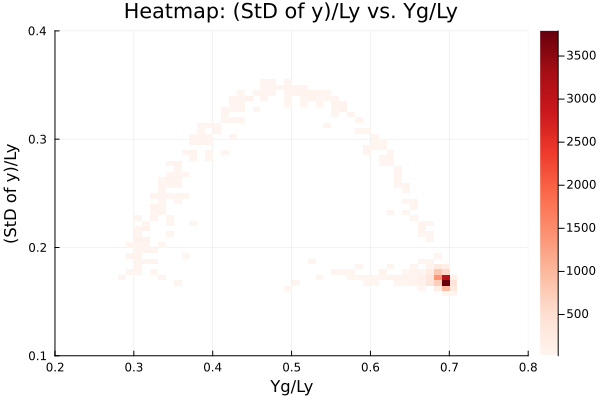
\includegraphics[width=\textwidth]{image/RaRtmap10_heat/2023-12-28T12:38:52.986_map_10times_chi1.265_Ay50_rho0.4_T0.43_dT0.04_Rd0.0_Rt0.5_Ra1.877538_g0.0003999718779659611_run4.0e8.png}
      \subcaption{Ra1.877,Rt0.5}
      \label{}
    \end{minipage} 
  \end{tabular}
  \caption{ヒートマップ, Ra固定}
  \label{}
\end{figure}

\begin{figure}[H]
  \centering
  \begin{tabular}{c}
    \begin{minipage}[t]{0.7\hsize}
      \centering
      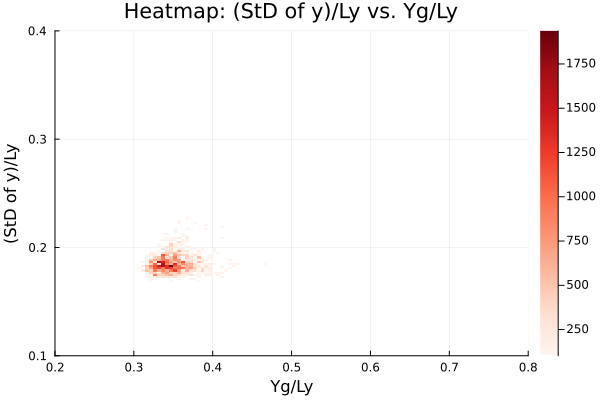
\includegraphics[width=\textwidth]{image/RaRtmap10_heat/2023-12-28T12:38:52.686_map_10times_chi1.265_Ay50_rho0.4_T0.43_dT0.04_Rd0.0_Rt0.5_Ra0.0_g0.0003999718779659611_run4.0e8.png}
      \subcaption{Ra0.0,Rt0.5}
      \label{}
    \end{minipage} \\
    \begin{minipage}[t]{0.7\hsize}
      \centering
      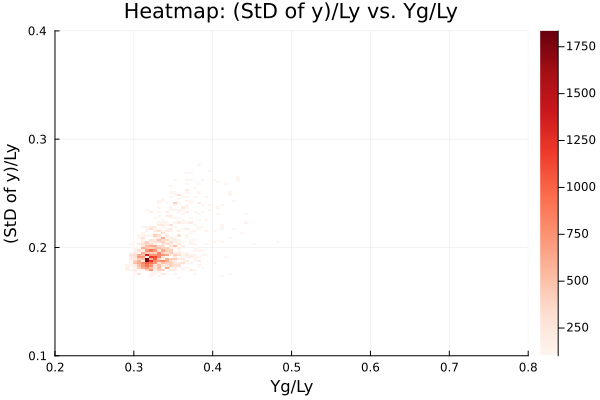
\includegraphics[width=\textwidth]{image/RaRtmap10_heat/2023-12-28T12:38:52.752_map_10times_chi1.265_Ay50_rho0.4_T0.43_dT0.04_Rd0.0_Rt0.5_Ra0.4693845_g0.0003999718779659611_run4.0e8.png}
      \subcaption{Ra0.469,Rt0.5}
      \label{}
    \end{minipage} \\
    \begin{minipage}[t]{0.7\hsize}
      \centering
      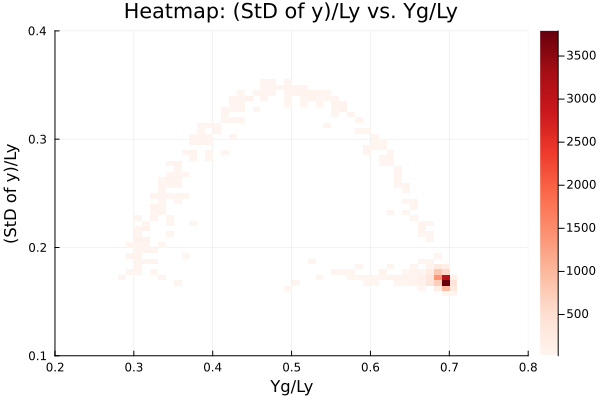
\includegraphics[width=\textwidth]{image/RaRtmap10_heat/2023-12-28T12:38:52.986_map_10times_chi1.265_Ay50_rho0.4_T0.43_dT0.04_Rd0.0_Rt0.5_Ra1.877538_g0.0003999718779659611_run4.0e8.png}
      \subcaption{Ra1.877,Rt0.5}
      \label{}
    \end{minipage} 
  \end{tabular}
  \caption{ヒートマップ, Rt固定}
  \label{}
\end{figure}

% 
\begin{figure}[H]
  \begin{tabular}{ccccc}
    \begin{minipage}[t]{0.2\hsize}
      \centering
      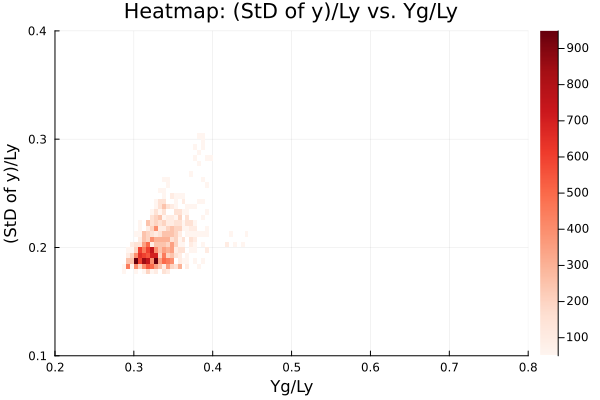
\includegraphics[width=\textwidth]{image/RaRtmap_heat/2023-11-14T18:19:29.358__chi1.265_Ay50_rho0.4_T0.43_dT0.04_Rd0.0_Rt0.0_Ra0.0_g0.0003999718779659611_run4.0e7_output.png}
      \subcaption{$\text{R}_\text{a}=0.0,\\\text{R}_\text{t}=0.0$}
      \label{fig:RaRtmap_heat_Ra0.0_Rt0.0}
    \end{minipage} &
    \begin{minipage}[t]{0.2\hsize}
      \centering
      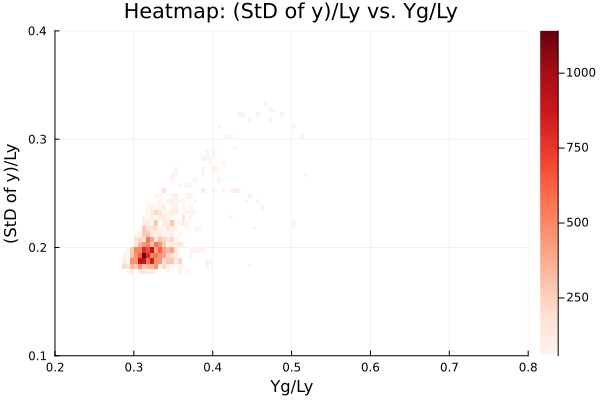
\includegraphics[width=\textwidth]{image/RaRtmap_heat/2023-11-14T19:14:52.710__chi1.265_Ay50_rho0.4_T0.43_dT0.04_Rd0.0_Rt0.0_Ra0.4693845_g0.0003999718779659611_run4.0e7_output.png}
      \subcaption{$\text{R}_\text{a}=0.469,\\\text{R}_\text{t}=0.0$}
      \label{}
    \end{minipage} &
    \begin{minipage}[t]{0.2\hsize}
      \centering
      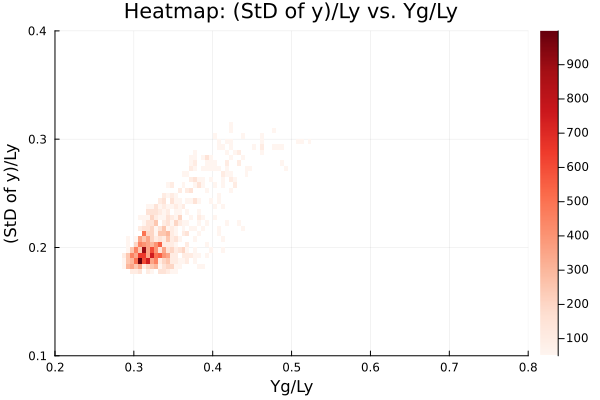
\includegraphics[width=\textwidth]{image/RaRtmap_heat/2023-11-14T20:07:58.625__chi1.265_Ay50_rho0.4_T0.43_dT0.04_Rd0.0_Rt0.0_Ra0.938769_g0.0003999718779659611_run4.0e7_output.png}
      \subcaption{$\text{R}_\text{a}=0.938,\\\text{R}_\text{t}=0.0$}
      \label{}
    \end{minipage} &
    \begin{minipage}[t]{0.2\hsize}
      \centering
      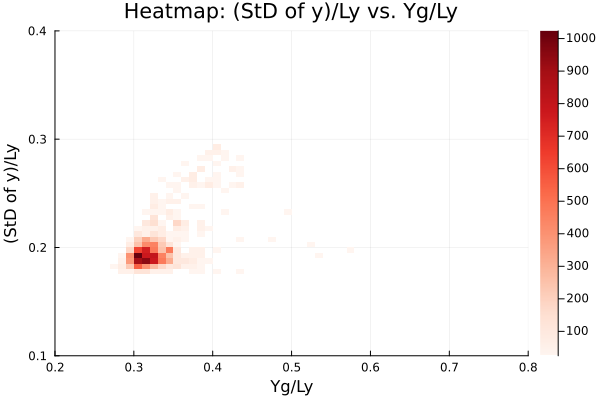
\includegraphics[width=\textwidth]{image/RaRtmap_heat/2023-11-14T21:01:09.992__chi1.265_Ay50_rho0.4_T0.43_dT0.04_Rd0.0_Rt0.0_Ra1.4081535_g0.0003999718779659611_run4.0e7_output.png}
      \subcaption{$\text{R}_\text{a}=1.408,\\\text{R}_\text{t}=0.0$}
      \label{}
    \end{minipage} &
    \begin{minipage}[t]{0.2\hsize}
      \centering
      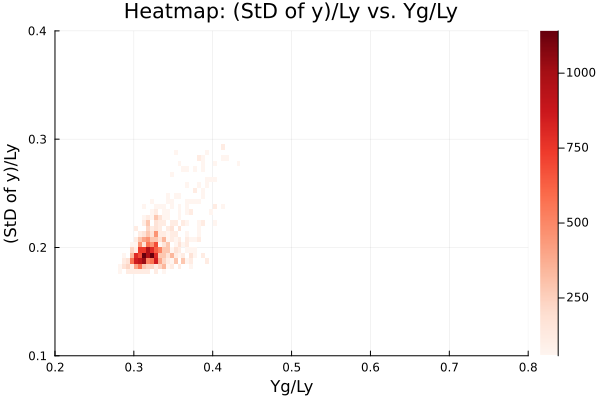
\includegraphics[width=\textwidth]{image/RaRtmap_heat/2023-11-14T21:54:59.835__chi1.265_Ay50_rho0.4_T0.43_dT0.04_Rd0.0_Rt0.0_Ra1.877538_g0.0003999718779659611_run4.0e7_output.png}
      \subcaption{$\text{R}_\text{a}=1.877,\\\text{R}_\text{t}=0.0$}
      \label{}
    \end{minipage} \\
    \begin{minipage}[t]{0.2\hsize}
      \centering
      \includegraphics[width=\textwidth]{image/RaRtmap_heat/2023-11-14T22:51:24.191__chi1.265_Ay50_rho0.4_T0.43_dT0.04_Rd0.0_Rt0.125_Ra0.0_g0.0003999718779659611_run4.0e7_output.png}
      \subcaption{$\text{R}_\text{a}=0.0,\\\text{R}_\text{t}=0.125$}
      \label{}
    \end{minipage} &
    \begin{minipage}[t]{0.2\hsize}
      \centering
      \includegraphics[width=\textwidth]{image/RaRtmap_heat/2023-11-14T23:48:31.439__chi1.265_Ay50_rho0.4_T0.43_dT0.04_Rd0.0_Rt0.125_Ra0.4693845_g0.0003999718779659611_run4.0e7_output.png}
      \subcaption{$\text{R}_\text{a}=0.469,\\\text{R}_\text{t}=0.125$}
      \label{}
    \end{minipage} &
    \begin{minipage}[t]{0.2\hsize}
      \centering
      \includegraphics[width=\textwidth]{image/RaRtmap_heat/2023-11-15T00:43:33.781__chi1.265_Ay50_rho0.4_T0.43_dT0.04_Rd0.0_Rt0.125_Ra0.938769_g0.0003999718779659611_run4.0e7_output.png}
      \subcaption{$\text{R}_\text{a}=0.938,\\\text{R}_\text{t}=0.125$}
      \label{}
    \end{minipage} &
    \begin{minipage}[t]{0.2\hsize}
      \centering
      \includegraphics[width=\textwidth]{image/RaRtmap_heat/2023-11-15T01:35:17.404__chi1.265_Ay50_rho0.4_T0.43_dT0.04_Rd0.0_Rt0.125_Ra1.4081535_g0.0003999718779659611_run4.0e7_output.png}
      \subcaption{$\text{R}_\text{a}=1.408,\\\text{R}_\text{t}=0.125$}
      \label{}
    \end{minipage} &
    \begin{minipage}[t]{0.2\hsize}
      \centering
      \includegraphics[width=\textwidth]{image/RaRtmap_heat/2023-11-15T02:27:34.337__chi1.265_Ay50_rho0.4_T0.43_dT0.04_Rd0.0_Rt0.125_Ra1.877538_g0.0003999718779659611_run4.0e7_output.png}
      \subcaption{$\text{R}_\text{a}=1.877,\\\text{R}_\text{t}=0.125$}
      \label{}
    \end{minipage} \\
    \begin{minipage}[t]{0.2\hsize}
      \centering
      \includegraphics[width=\textwidth]{image/RaRtmap_heat/2023-11-15T03:19:32.715__chi1.265_Ay50_rho0.4_T0.43_dT0.04_Rd0.0_Rt0.25_Ra0.0_g0.0003999718779659611_run4.0e7_output.png}
      \subcaption{$\text{R}_\text{a}=0.0,\\\text{R}_\text{t}=0.250$}
      \label{}
    \end{minipage} &
    \begin{minipage}[t]{0.2\hsize}
      \centering
      \includegraphics[width=\textwidth]{image/RaRtmap_heat/2023-11-15T04:11:00.956__chi1.265_Ay50_rho0.4_T0.43_dT0.04_Rd0.0_Rt0.25_Ra0.4693845_g0.0003999718779659611_run4.0e7_output.png}
      \subcaption{$\text{R}_\text{a}=0.469,\\\text{R}_\text{t}=0.250$}
      \label{}
    \end{minipage} &
    \begin{minipage}[t]{0.2\hsize}
      \centering
      \includegraphics[width=\textwidth]{image/RaRtmap_heat/2023-11-15T05:03:45.973__chi1.265_Ay50_rho0.4_T0.43_dT0.04_Rd0.0_Rt0.25_Ra0.938769_g0.0003999718779659611_run4.0e7_output.png}
      \subcaption{$\text{R}_\text{a}=0.938,\\\text{R}_\text{t}=0.250$}
      \label{}
    \end{minipage} &
    \begin{minipage}[t]{0.2\hsize}
      \centering
      \includegraphics[width=\textwidth]{image/RaRtmap_heat/2023-11-15T05:53:00.667__chi1.265_Ay50_rho0.4_T0.43_dT0.04_Rd0.0_Rt0.25_Ra1.4081535_g0.0003999718779659611_run4.0e7_output.png}
      \subcaption{$\text{R}_\text{a}=1.408,\\\text{R}_\text{t}=0.250$}
      \label{}
    \end{minipage} &
    \begin{minipage}[t]{0.2\hsize}
      \centering
      \includegraphics[width=\textwidth]{image/RaRtmap_heat/2023-11-15T06:43:21.554__chi1.265_Ay50_rho0.4_T0.43_dT0.04_Rd0.0_Rt0.25_Ra1.877538_g0.0003999718779659611_run4.0e7_output.png}
      \subcaption{$\text{R}_\text{a}=1.877,\\\text{R}_\text{t}=0.250$}
      \label{}
    \end{minipage} \\
    \begin{minipage}[t]{0.2\hsize}
      \centering
      \includegraphics[width=\textwidth]{image/RaRtmap_heat/2023-11-15T07:34:00.555__chi1.265_Ay50_rho0.4_T0.43_dT0.04_Rd0.0_Rt0.375_Ra0.0_g0.0003999718779659611_run4.0e7_output.png}
      \subcaption{$\text{R}_\text{a}=0.0,\\\text{R}_\text{t}=0.375$}
      \label{}
    \end{minipage} &
    \begin{minipage}[t]{0.2\hsize}
      \centering
      \includegraphics[width=\textwidth]{image/RaRtmap_heat/2023-11-15T08:24:37.362__chi1.265_Ay50_rho0.4_T0.43_dT0.04_Rd0.0_Rt0.375_Ra0.4693845_g0.0003999718779659611_run4.0e7_output.png}
      \subcaption{$\text{R}_\text{a}=0.469,\\\text{R}_\text{t}=0.375$}
      \label{}
    \end{minipage} &
    \begin{minipage}[t]{0.2\hsize}
      \centering
      \includegraphics[width=\textwidth]{image/RaRtmap_heat/2023-11-15T09:16:40.082__chi1.265_Ay50_rho0.4_T0.43_dT0.04_Rd0.0_Rt0.375_Ra0.938769_g0.0003999718779659611_run4.0e7_output.png}
      \subcaption{$\text{R}_\text{a}=0.938,\\\text{R}_\text{t}=0.375$}
      \label{}
    \end{minipage} &
    \begin{minipage}[t]{0.2\hsize}
      \centering
      \includegraphics[width=\textwidth]{image/RaRtmap_heat/2023-11-15T10:07:20.945__chi1.265_Ay50_rho0.4_T0.43_dT0.04_Rd0.0_Rt0.375_Ra1.4081535_g0.0003999718779659611_run4.0e7_output.png}
      \subcaption{$\text{R}_\text{a}=1.408,\\\text{R}_\text{t}=0.375$}
      \label{}
    \end{minipage} &
    \begin{minipage}[t]{0.2\hsize}
      \centering
      \includegraphics[width=\textwidth]{image/RaRtmap_heat/2023-11-15T10:59:30.665__chi1.265_Ay50_rho0.4_T0.43_dT0.04_Rd0.0_Rt0.375_Ra1.877538_g0.0003999718779659611_run4.0e7_output.png}
      \subcaption{$\text{R}_\text{a}=1.877,\\\text{R}_\text{t}=0.375$}
      \label{}
    \end{minipage} \\
    \begin{minipage}[t]{0.2\hsize}
      \centering
      \includegraphics[width=\textwidth]{image/RaRtmap_heat/2023-11-15T11:53:37.697__chi1.265_Ay50_rho0.4_T0.43_dT0.04_Rd0.0_Rt0.5_Ra0.0_g0.0003999718779659611_run4.0e7_output.png}
      \subcaption{$\text{R}_\text{a}=0.0,\\\text{R}_\text{t}=0.500$}
      \label{}
    \end{minipage} &
    \begin{minipage}[t]{0.2\hsize}
      \centering
      \includegraphics[width=\textwidth]{image/RaRtmap_heat/2023-11-15T12:45:26.303__chi1.265_Ay50_rho0.4_T0.43_dT0.04_Rd0.0_Rt0.5_Ra0.4693845_g0.0003999718779659611_run4.0e7_output.png}
      \subcaption{$\text{R}_\text{a}=0.469,\\\text{R}_\text{t}=0.500$}
      \label{fig:RaRtmap_heat_Ra0.469_Rt0.500}
    \end{minipage} &
    \begin{minipage}[t]{0.2\hsize}
      \centering
      \includegraphics[width=\textwidth]{image/RaRtmap_heat/2023-11-15T13:37:58.058__chi1.265_Ay50_rho0.4_T0.43_dT0.04_Rd0.0_Rt0.5_Ra0.938769_g0.0003999718779659611_run4.0e7_output.png}
      \subcaption{$\text{R}_\text{a}=0.938,\\\text{R}_\text{t}=0.500$}
      \label{fig:RaRtmap_heat_Ra0.938_Rt0.500}
    \end{minipage} &
    \begin{minipage}[t]{0.2\hsize}
      \centering
      \includegraphics[width=\textwidth]{image/RaRtmap_heat/2023-11-15T14:30:22.529__chi1.265_Ay50_rho0.4_T0.43_dT0.04_Rd0.0_Rt0.5_Ra1.4081535_g0.0003999718779659611_run4.0e7_output.png}
      \subcaption{$\text{R}_\text{a}=1.408,\\\text{R}_\text{t}=0.500$}
      \label{}
    \end{minipage} &
    \begin{minipage}[t]{0.2\hsize}
      \centering
      \includegraphics[width=\textwidth]{image/RaRtmap_heat/2023-11-15T15:21:59.073__chi1.265_Ay50_rho0.4_T0.43_dT0.04_Rd0.0_Rt0.5_Ra1.877538_g0.0003999718779659611_run4.0e7_output.png}
      \subcaption{$\text{R}_\text{a}=1.877,\\\text{R}_\text{t}=0.500$}
      \label{}
    \end{minipage} 
  \end{tabular}
  \caption{$t_i = 4.0 \times 10^4, t_f = 2.0 \times 10^5, \dd t \sqrt{\varepsilon / m \sigma^2}= 0.005, t \sqrt{\varepsilon / m \sigma^2} = 200 ごとにプロット.$}
  \label{}
\end{figure}



